\todo{General comments
	
	- connect your sentences
	(look up sentence connectors)
	
	- browse the web about how to write introductions
	
	- NEW
	you have too much text per page :-)
	For a more professional look and a better reading experience: make your font large enough, make the distance between lines large enough, put some extra distance between paragraphs.}

\todo{where do you cover track reconstruction, local calorimeter reconstruction, local muon reconstruction?}

\todo{I recommend to move the information of this chapter as follows:
	
	General information about particle reconstruction, (reconstruction algorithms and reconstruction quality) belongs to the chapter about CMS. 
	
	The description of the specific object definitions you employed belong to the analysis chapter.
	
	A simpler title would simply be
	“particle reconstruction”}

\todo{start this chapter / section by explaining what is to be accomplished 
	(studying final states of collisions) and what the strategy is (reconstruction of all particles in the final state, which allows doing jets, letpon isolation, …)}



\section{The Particle Flow Algorithm}

\todo{This is my idea about how one should describe the particle flow:
	
	You need to give an idea of the basic idea behind the particle flow algorithm:
	
	- what information does the algorithm use for input (tracks, calorimeter hits, calorimeter clusters, muon hits, muon segments,….)
	- what are the basic steps of the algorithm
	- how is the input information filtered at each step
	
	no need to go in great detail, but the reader should get an idea.
	
	Consult Christian before taking action.}

The raw data collected by the CMS experiment is the input of a detailed offline reconstructions of the collision final states. CMS developed over the years an algorithm, called the Particle Flow (PF) \cite{CMS:2009nxa,CMS:2010byl}, that attempts to identify and to reconstruct the kinematic properties of each of the particles in the final states. For this purpose all the information coming from each of the CMS subdetectors is combined. This algorithm heavily relies on the precise measurement of the momenta of charged particles with the silicon tracker, and the precise measurement of photon and electron energies with the highly granular and hermetic ECAL, to overcome the coarser granularity of the HCAL. The reconstructed particles are then used to reconstruct jets, \hadtau candidates, and the vector imbalance in transverse momentum in the event, referred to as \ptvecmiss, as well as to quantify the isolation of leptons. 

\subsection{Electrons reconstruction}

\todo{last sentence is probably only relevant in the object definition section of your analysis chapter, unless the BDT is used inside the particle flow (could well be)}

Electrons are reconstructed by matching tracks in the inner detector with energy depositions in the ECAL \cite{CMS:2009nxa,Baffioni2007}. The tracks of electron candidates are reconstructed using a Gaussian sum filter \cite{Adam:2005bya} algorithm, which accounts for the emission of bremsstrahlung photons along the electron trajectory. Energy loss in bremsstrahlung is reconstructed by searching for energy depositions in the ECAL located in directions tangential to the electron track. A multivariate approach based on boosted decision trees (BDT) \cite{Hocker:2007ht} is employed for electron identification \cite{1748-0221-10-06-P06005}.

\subsection{Muons reconstruction}

 The identification of muons is based on linking track segments reconstructed in the silicon tracking detector and in the muon system \cite{Chatrchyan:2012xi}. The matching between track segments is done outside-in, starting from a track in the muon system, and inside-out, starting from a track reconstructed in the inner detector. In case a link can be established, the track parameters are refitted using the combined hits in the inner and outer detectors, with the resulting track referred to as a global muon track. \todo{last sentence is probably only relevant in the object definition section of your analysis chapter, unless the ID is used inside the particle flow (could well be)}Quality criteria are applied on the multiplicity of hits, on the number of matched segments, and on the fit quality of the global muon track, quantified through a \ensuremath{\chisquare}.

\todo{you need a subsection about hadrons and photons}

\subsection {The Jet reconstruction}

\todo{Jet reconstruction does not belong to the particle flow algorithm. Probably you want to have the section about jets in the object definition section of your analysis chapter. You might want a few words and figures about jets in the particle reconstruction section of the CMS section}

\todo{paragraphs in this subsection are too long, they cover too many topics}

Jets within the range \ensuremath{|\eta| < 4.7} are reconstructed using the anti-\ensuremath{k_{T}} algorithm \cite{antikt} with a distance parameter of 0.5. As mentioned previously,the particles reconstructed by the PF algorithm are used as input to the jet reconstruction. Reconstructed jets are required not to overlap with identified electrons, muons, or \hadtau within \ensuremath{\deltar < 0.5}, and to pass two levels of jet identification criteria: (i) misidentified jets, mainly generating from calorimeter noise, are rejected by requiring reconstructed jets to pass a set of loose jet identification criteria \cite{CMS:2010xta} and (ii) jets originating from pileup interactions are rejected through an MVA-based jet identification discriminant, based on information about the vertex and energy distribution within the jet \cite{CMS:2013wea}. The energy of reconstructed jets is calibrated as a function of jet \pt and \ensuremath{\eta} \cite{1748-0221-6-11-P11002}. A display of a simple hadronic jet in the $(x, y)$ view and in the $(\eta,\phi)$ view, on the ECAL surface and the HCAL surface is available on Figure 	\ref{fig:PF_event_display}. The contribution of pileup to the energy of jets originating from the hard scattering is compensated by determining a median transverse momentum density (\ensuremath{\rho}) for each event, and subtracting the product of (\ensuremath{\rho}) times the area of the jet, computed in the \ensuremath{\eta-\Phi} plane,from there constructed jet \pt \cite{Cacciari:2008gn, Cacciari:2007fd}. Jets originating from the hadronization of b quarks are identified through the combined secondary vertex (CSV) algorithm \cite{Chatrchyan:2012jua}, which exploits observables related to the long lifetime of b hadrons and the higher particle multiplicity and mass of b jets compared to light-quark and gluon jets.

\todo{This is more or less an orphaned figure. You don’t /hardly describe anything about it in the text. At least clarify in the text why you show the figure, what should the reader learn from it?}

\begin{figure}
	\centering
	\begin{subfigure}{0.9\textwidth}
		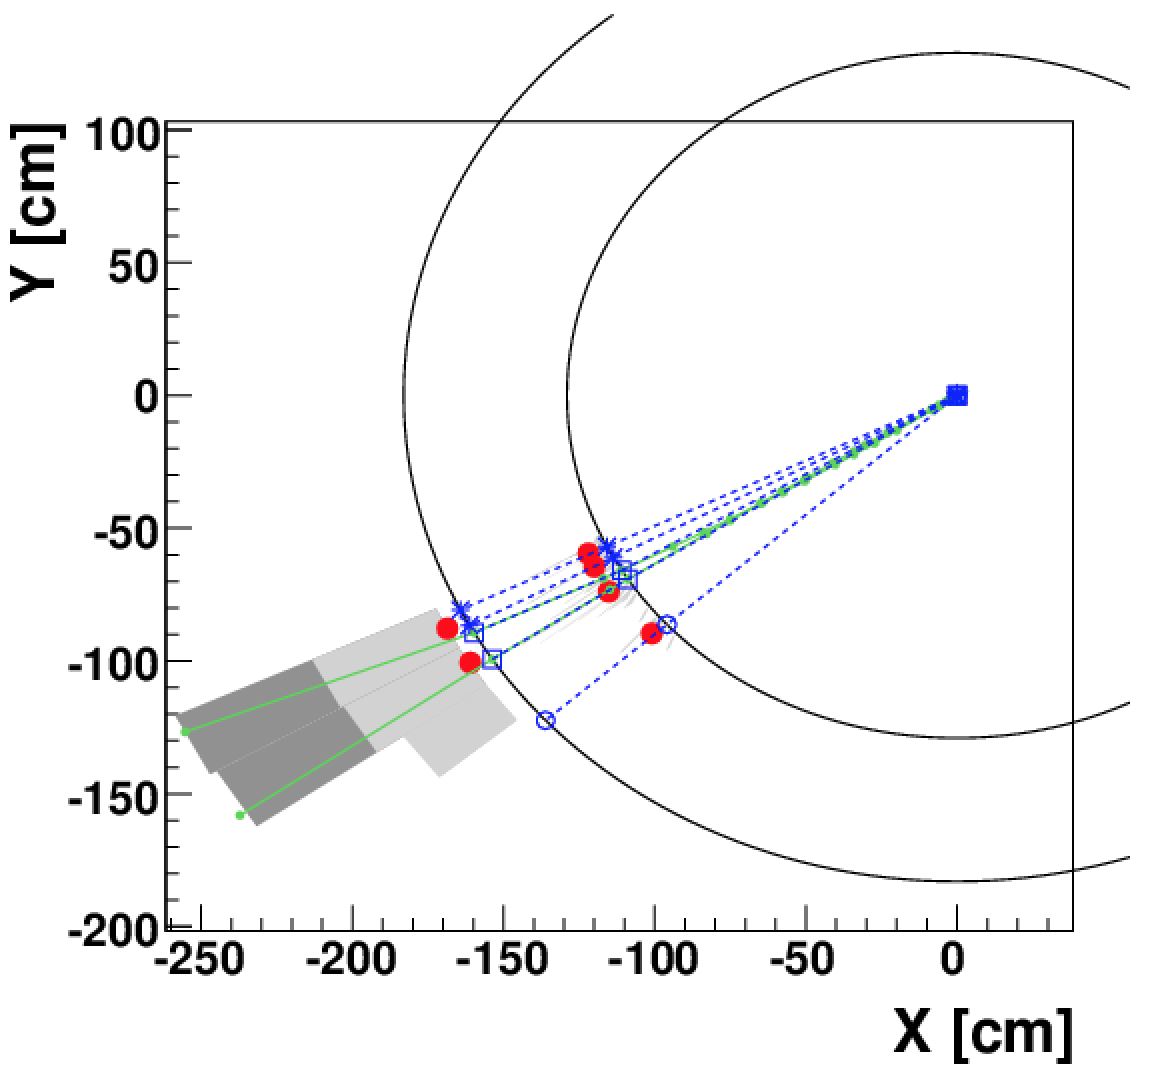
\includegraphics[width=.8\linewidth]{analysis/pics/PF_a.png}
		\caption{The $(x, y)$ view.}
		\label{fig:PF_a}
	\end{subfigure}
	
	\begin{subfigure}{.4\textwidth}
		\centering
		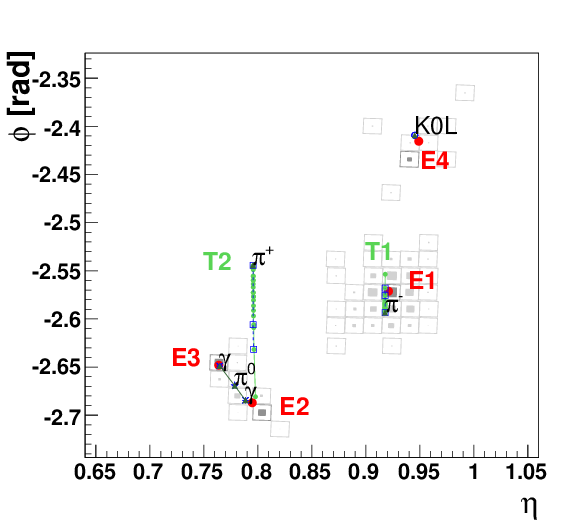
\includegraphics[width=.8\linewidth]{analysis/pics/PF_b.png}
		\caption{The $(\eta,\phi)$ view on ECAL.}
		\label{fig:PF_b}
	\end{subfigure}
	\begin{subfigure}{.4\textwidth}
		\centering
		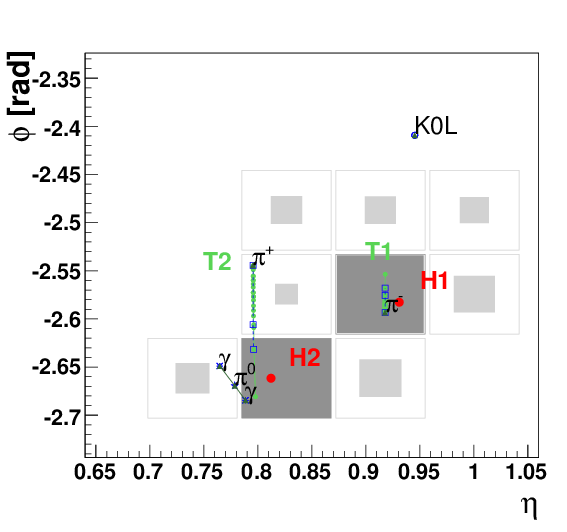
\includegraphics[width=.8\linewidth]{analysis/pics/PF_c.png}
		\caption{The $(\eta,\phi)$ view on HCAL.}
		\label{fig:PF_c}
	\end{subfigure}%
	\caption{An event display of a simple hadronic jet in the $(x, y)$ view (Figure \ref{fig:PF_a}) and in the $(\eta,\phi)$ view, where $\eta$ stands for pseudo-rapidity and $\phi$ for the azimuthal angle, on the ECAL surface (Figure \ref{fig:PF_b}) and the HCAL surface (Figure \ref{fig:PF_c}). (These two surfaces are represented as two circles centered around the interaction point in the first view.) The $K^{0}_{L}$, the $\pi^{-}$ and the two photons from the $\pi^{0}$ decay are detected as four well separated ECAL clusters (Figure \ref{fig:PF_b}). The $\pi^{+}$ leaves no energy in the ECAL. The two charged pions are reconstructed as charged-particle tracks, appearing as vertical solid lines in the $(\eta,\phi)$ views and circular arcs in the $(x, y)$ view. These tracks point towards two HCAL clusters (Figure \ref{fig:PF_c}). In all three views, the cluster positions are represented by dots, the simulated particles by dashed lines, and the position of their impact on the calorimeter surfaces by various open markers.}
	\label{fig:PF_event_display}
\end{figure}

\todo{MET and MET-like variables belong to the object definition section of the analysis chapter 
	
	you say MET and |sum p_T^jet| are  the same, while they are not
	
	besides, MET does not belong to a section  named “jet reconstruction”
	
	do you use the multivariate technique in [26]? if not don’t mention it}

Two algorithms are used to reconstruct \ptvecmiss, the imbalance in transverse momentum in the event, whose magnitude is referred to as \met. The standard algorithm computes the negative vectorial sum of all particle momenta reconstructed using the PF algorithm. In addition, a multivariate regression algorithm \cite{Khachatryan:2014gga} has been developed to reduce the effect of pileup on the resolution in \met. The algorithm utilizes the fact that pileup predominantly produces jets of low \pt, while leptons and high-\pt jets are produced almost exclusively in the hard-scatter. The transverse mass, \mt, of the system constituted by an electron or a muon and \met is used to either select or remove events that are due to W+jets and tt production. 

\clearpage

\section {The Tau Lepton}

\todo{i don’t like subsubsections, and you don’t need them anyway:
	section{tau lepton reconstruction}
	subsection{intruduction}
	subsection{reconstruction algorithm}
	subsection{isolation}
	subsection{electron and muon veto}
	}

The $\tau$ lepton was discovered between 1974 and 1977 by the team under Martin Perl while studying the $e^{+}+e^{-}\longrightarrow e^{\pm}+\mu^{\mp}$. With a mean lifetime of $2.9\times10^{−13}$ s and a mass of 1776.82 \mev \cite{Agashe:2014kda} is the heaviest of the leptons, enough to decay into hadrons, and it does so in about two thirds of the cases, typically into either one or three charged pions or kaons and up to two neutral pions \ensuremath{\pi^{0}}, and one neutrino \ensuremath{\nu_{\tau}}. The \ensuremath{\pi^{0}} meson decays almost exclusively into \ensuremath{\gamma\gamma}. Among all the possible hadronic decays as shown on Table \ref{table:tau_hdecay} the ones called "one-prong", where only one charged hadron is produced, are the most frequent. The $\tau$ decays also leptonically, with a branching ratio of $17\%$ for each channel, via the following decay $\tau\longrightarrow\nu_{\tau}W^{*}\longrightarrow\nu_{\tau}l\nu_{l}$.

\begin{figure}[tbh!]
	\begin{center}	
		\begin{tabular}{ | c | c | c | c |}
			\hline
			Decay Mode & Resonance & Mass [\mev] & BF (\%) \\ \hline
			\hline
			$\tau^{-}\longrightarrow h^{-}\nu_{\tau}$& $\pi$ & 139.6 & 11.6 \\ \hline
			$\tau^{-}\longrightarrow h^{-}\pi^{0}\nu_{\tau}$& $\rho$ & 770 & 26.0 \\ \hline
			%				$\tau^{-}\longrightarrow h^{-}\pi^{0}\pi^{0}\nu_{\tau}$ & $a_{1}$ & 1200 & \\ 10.8 \hline
			$\tau^{-}\longrightarrow h^{-} h^{+} h^{-} \nu_{\tau}$& $a_{1}$& 1200 & 9.8 \\ \hline
			$\tau^{-}\longrightarrow h^{-} h^{+} h^{-} \pi^{0}\nu_{\tau}$& & & 4.8 \\ \hline
			other hadronic channels& & & 1.7 \\ \hline
			\hline
			total & & & 64.8 \\ \hline
			\hline
		\end{tabular}
		\caption{ Hadronic tau decay modes into either one or three charged hadrons h and potential $\pi_{0}$, and the corresponding branching fractions BF. Also shown are the intermediate resonances and their masses, which are used in some of the tau reconstruction algorithms.}
		\label{table:tau_hdecay}
	\end{center}
\end{figure}

\subsection{Algorithm for hadronic Tau reconstruction and identification}
The \hadtau decays are reconstructed and identified using the hadrons-plus-strips (HPS) algorithm \cite{Chatrchyan:2012zz}, a cut-based algorithm focusing on the reconstruction of neutral pions. The HPS algorithm is seeded by jets of \ensuremath{\pt > 14 \gev} and \ensuremath{|\eta| < 2.5}, reconstructed using the anti-\ensuremath{k_{T}} algorithm \cite{antikt} with a distance parameter of 0.5. The algorithm is designed to reconstruct individual decay modes of the \ensuremath{\tau} lepton, taking advantage of the excellent performance of the PF algorithm in reconstructing individual charged and neutral particles.
The reconstruction and identification of \hadtau decays in the HPS algorithm is performed in two steps:

\begin{itemize}
	\item \textbf{Reconstruction:} combinations of charged and neutral particles reconstructed by the PF algorithm that are compatible with specific \hadtau decays are constructed, and the four-momentum, expressed in terms of (\pt, \ensuremath{\eta}, \ensuremath{\phi} , and mass) of \hadtau candidates, is computed.
	
	\item \textbf{Identification:} discriminators that separate \hadtau decays from quark and gluon jets, and from electrons and muons, are computed. This provides a reduction in the jet \ensuremath{\longrightarrow \hadtau}, \ensuremath{e \longrightarrow \hadtau}, and \ensuremath{\mu \longrightarrow \hadtau} misidentification rates.
\end{itemize}

\subsubsection{Identification of decay modes}

Reconstruction of specific \hadtau decay modes requires reconstruction of neutral pions that are present in most of the hadronic \ensuremath{\tau} decays. The high probability for photons originating from \ensuremath{\pi^{0} \longrightarrow \gamma \gamma} decays to convert to \ensuremath{e^{+}e^{-}} pairs within the volume of the CMS tracking detector is taken into account by clustering the photon and electron constituents of the \ensuremath{\tau}-seeding jet into “strips” in the \ensuremath{\eta - \phi} plane. The clustering of electrons and photons of \ensuremath{\pt > 0.5} \gev into strips proceeds via an iterative procedure. The electron or photon of highest \pt not yet included into any strip is used to seed a new strip. The initial position of the strip in the \ensuremath{\eta - \phi} plane is set according to the \ensuremath{\eta} and \ensuremath{\phi} of the seed \ensuremath{e} or \ensuremath{\gamma}. The \ensuremath{e} or \ensuremath{\gamma} of next-highest \pt that is within an \ensuremath{\eta \times \phi} window centred on the strip location is merged into the strip. The strip position is then recomputed as an energy-weighted average of all electrons and photons contained in the strip \cite{Khachatryan:2015dfa}.

\hadtau candidates are formed by combining the strips with the charged-particle constituents of the jet. The charged particles are required to satisfy the condition \ensuremath{\pt > 0.5 \gev}. The distance of closest approach between their tracks and the hypothetical production vertex of the \hadtau candidate, taken to be the vertex closest to the charged particle of highest \pt within the jet, is required to be less than 0.4 cm in the z direction and \ensuremath{< 0.03} cm in the transverse plane. These requirements removes spurious reconstructed tracks and significantly reduces the effect of pileup.

A combinatorial approach is taken for constructing hadronic \ensuremath{\tau} candidates. Multiple \hadtau hypotheses, corresponding to combinations of either one or three charged particles and up to two strips, are constructed for each jet.

The four-momentum of each \hadtau candidate hypothesis (\pt, \ensuremath{\eta}, \ensuremath{\phi}, and mass) is given by the four- momentum sum of the charged particles and strips. In a few per cent of the cases, the charged particles included in the \hadtau candidates are identified as electrons or muons, and are assigned their respective electron or muon masses by the PF algorithm. The HPS algorithm sets the mass of all charged particles included in \hadtau candidates to that of the charged pion, except for electron constituents of strips, which are treated as massless. The charge of \hadtau candidates is reconstructed by summing the charges of all particles included in the construction of the \hadtau candidate, except for the electrons contained in strips. The probability for mis-reconstructing the \hadtau charge is \ensuremath{\approx 1 \%}, with a moderate dependence on \pt and \ensuremath{\eta}, for taus from Z decays.

\begin{figure}[tbh!]
	\centering
	\begin{tabular}{cc}
		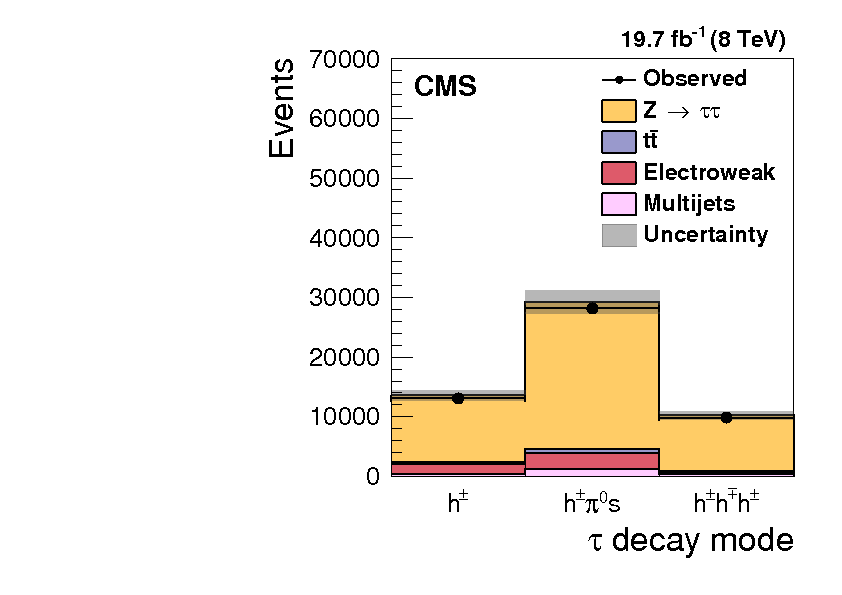
\includegraphics[width=0.45\textwidth]{objreconstruction/pics/scalefactors050314.png}
		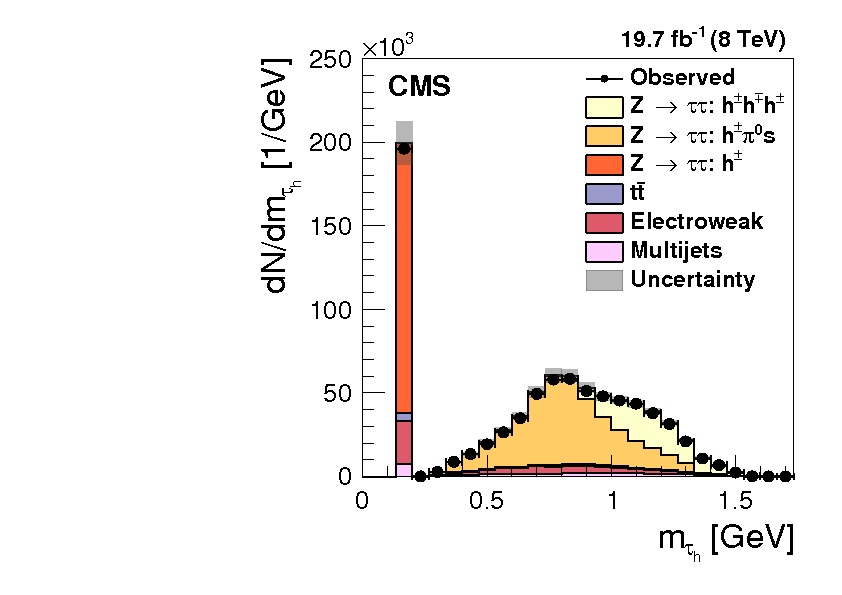
\includegraphics[width=0.45\textwidth]{objreconstruction/pics/plots_paper_tauIdAlgorithm_ZTT_mTau_ZTT_linear.png} 		
	\end{tabular}
	\caption{Distributions in (left) reconstructed \hadtau decay modes and (right) \hadtau candidate masses in \ensuremath{Z/\gamma^{*} \longrightarrow \tau\tau}  events selected in data, compared to MC expectations. The \ensuremath{Z/\gamma^{*} \longrightarrow \tau\tau}  events are selected in the decay channel of muon and \hadtau \cite{Khachatryan:2015dfa}.}
	\label{fig:Ztautau_decaymodes}
\end{figure}

The following criteria are applied to assure the compatibility of each hypothesis with the signatures expected for the different \hadtau decays in Table \ref{table:tau_hdecay}:

\begin{enumerate}
	\item \ensuremath{h^{\pm}h^{\pm}h^{\pm}}: Combination of three charged particles with mass \ensuremath{0.8 < m_{\hadtau} < 1.5 \gev}. The tracks are required to originate within \ensuremath{\Delta z < 0.4} cm of the same event vertex, and to have a total charge of one.
	\item \ensuremath{h^{\pm}\pi^{0}\pi^{0}}: Combination of a single charged particle with two strips. The mass of the \hadtau candidate is required to satisfy the condition \ensuremath{0.4 < m_{\hadtau} < 1.2 \sqrt{\pt [\gev]/100}}\gev. The size of the mass window is enlarged for \hadtau candidates of high \pt to account for resolution effects. The upper limit on the mass window is constrained to be at least 1.2 and at most 4.0 \gev.
	\item \ensuremath{h^{\pm}\pi^{0}}: Combination of one charged particle and one strip with mass \ensuremath{0.3 < m_{\hadtau} < 1.3 \sqrt{\pt [\gev]/100}}\gev. The upper limit on the mass window is constrained to be at least 1.3 and at most 4.2 \gev.
	\item \ensuremath{h^{\pm}}: A single charged particle without any strips.
\end{enumerate}

The combinations of charged particles and strips considered by the HPS algorithm represent all hadronic \ensuremath{\tau} decay modes in Table \ref{table:tau_hdecay}, except \ensuremath{τ^{-} \longrightarrow h^{-}h^{+}h^{-}\pi^{0}\nu_{\tau}}. The latter corresponds to a branching fraction of \ensuremath{4.8\%} and is not considered in the present version of the algorithm, because of its contamination by jets. The \ensuremath{h^{\pm}\pi^{0}} and \ensuremath{h^{\pm}\pi^{0}\pi^{0}} decays are analyzed together, and referred to as \ensuremath{h^{\pm}\pi^{0}s}.

Hypotheses that fail the mass window selection for the corresponding decay mode are discarded. When multiple combinations of charged hadrons and strips pass the mass window and the signal cone requirements, the hypothesis for the candidate with largest \pt is retained. All other combinations are discarded, resulting in a unique \hadtau candidate to be associated to each jet.

\todo{you should make clear why the rho and a1 resonances are there.}

\todo{what about quoting an efficiency here?}

The distributions in the decay modes and in the mass of \hadtau candidates in \ensuremath{Z/\gamma^{*} \longrightarrow \tau\tau} events are shown in Figure \ref{fig:Ztautau_decaymodes}. The contribution of the \ensuremath{Z/\gamma^{*} \longrightarrow \tau\tau} signal is split according to the reconstructed \hadtau mode, as shown in the legend. For \hadtau candidates reconstructed in the \ensuremath{h^{\pm}\pi^{0}s} and \ensuremath{h^{\pm}h^{\pm}h^{\pm}} modes, the \ensuremath{m_{\hadtau}} distribution peaks near the intermediate \ensuremath{ρ\rho(770)} and \ensuremath{a_{1}(1260)} meson resonances (cf. Table \ref{table:tau_hdecay}), as expected. The narrow peak at the charged pion mass is due to \hadtau candidates reconstructed in the \ensuremath{h^{\pm}} mode.

\subsubsection{Tau-isolation discriminants}

\todo{isolation reference should come earlier in the subsection}

\todo{I don’t think “cutoff-based selection” is a proper expression
	
	do you need to describe both the cut-based and the MVA discriminant? Only mention the one(s) you use.}

Requiring reconstructed \hadtau candidates to pass strict isolation requirements constitutes the main handle for reducing the large multijet background. Tau leptons are usually isolated relative to other particles in the event, and so are their decay products, in contrast to quark and gluon jets. Two types of \hadtau isolation discriminants have been developed, using simple cutoff-based selections and an MVA approach. The expected efficiency of the \hadtau isolation discriminants in \ensuremath{Z/\gamma^{*} \longrightarrow \tau\tau} events goes from \ensuremath{49.0\%} (Loose) to \ensuremath{38.1}\% (Tight) for the cutoff-based approach and \ensuremath{55.9\%} (Very Loose) to \ensuremath{27.3\%} (Tight) for the MVA one. \todo{just “rate”, not “rate efficiency”
	
	how is the rate defined? it’s really not clear from the text what these numbers mean.}The Jet \ensuremath{\to \tau} misidentification rate efficiency of the \hadtau isolation discriminants in Multi-jet events goes from \ensuremath{3.86 \times 10^{−3}} (Loose) to \ensuremath{1.75 \times 10^{−3}}\% (Tight) for the cutoff-based approach and \ensuremath{6.21 \times 10^{−3}} (Very Loose) to \ensuremath{4.43 \times 10^{−3}} (Tight) for the MVA one \cite{Khachatryan:2015dfa}.
 
\subsubsection{Discriminants against electrons and muons}

\todo{rate is not defined

note there is a rate > 1
i don’t know whether this is correct,
cause I don’t understand the rate definition.

cutoff-based -> cut based

avoid mentioning both MVA and cut-based. only mention the ones you use.

you need references for the discriminators earlier in the subsection}

Electrons and muons have a sizable probability to get reconstructed in the \ensuremath{h^{\pm}} decay mode. Electrons radiating a bremsstrahlung photon that subsequently converts may also get reconstructed in the \ensuremath{h^{\pm}\pi^{0}s} decay mode. In particular, electrons and muons originating from decays of W and Z bosons, which are produced with cross sections of \ensuremath{\approx100} nb at the LHC at \ensuremath{\sqrt{s} = 8} \tev have a high chance to pass isolation-based \hadtau identification criteria. Dedicated discriminants have been developed to separate \hadtau from electrons and muons. The separation of \hadtau from electrons is based on an MVA approach, with an efficiency and \ensuremath{e\to \tau} misidentification rate going from \ensuremath{93.3\%} and \ensuremath{2.38 \times 10^{−2}} (Very loose) to \ensuremath{72.1\%} and \ensuremath{3.54 \times 10^{−4}} (Very tight) in \ensuremath{Z/\gamma^{*} \longrightarrow \tau\tau} events.
A cutoff-based and an MVA based discriminant are used to separate \hadtau from muons. The expected efficiency of the \hadtau against muon discriminants in \ensuremath{Z/\gamma^{*} \longrightarrow \tau\tau} events goes from \ensuremath{99.3\%} (Loose) to \ensuremath{99.1}\% (Tight) for the cutoff-based approach and \ensuremath{99.5\%} (Loose) to \ensuremath{98\%} (Tight) for the MVA one. The \ensuremath{\mu \to \tau} misidentification rate efficiency of the \hadtau isolation discriminants in \ensuremath{Z/\gamma^{*} \longrightarrow \mu\mu} events goes from \ensuremath{1.77 \times 10^{−3}} (Loose) to \ensuremath{7.74 \times 10^{−4}}\% (Tight) for the cutoff-based approach and \ensuremath{5.20 \times 10^{−4}} (Loose) to \ensuremath{3.18 \times 10^{−4}} (Tight) for the MVA one \cite{Khachatryan:2015dfa}.

\section {Analysis Physics Objects}

\subsection{Primary Vertices}
\label{subsec::objsel_vertex}

\todo{belongs to event reconstruction in the CMS chapter}

The determination of collisions Primary Vertices (PV) for each of the bunch crossing is critical for reducing pile up effects and to detect long lived particles such as mesons. CMS reconstructs PVs starting from the vertices of all well reconstructed charged particle tracks in the event \cite{CMS-PAS-TRK-10-005}. The first step consist on clustering the tracks according to the position on the z-axis of their closest track segment with respect to the beam line \cite{CMS-IN-2011-014}. Then, a PV is reconstructed from each cluster with two or more constituents using a dedicated fit procedure. Which PV corresponds to the hardest interaction in the event is determined based on the tracks associated to the PV. The transverse momenta of all tracks associated to the PV are summed and the vertex with the highest sum is chosen. Every event used in this analysis requires at least a reconstructed PV. Table~\ref{table:vertexobjdefinition} shows the detailed selection criteria for such requirement.

\subsection{Tau}
\label{subsec::objsel_tau}

\todo{hm, you write 4.3.2 as if 4.2 does not exist
	
	refer back to the section about taus (4.2)
	
	4.2 and 4.3.2 are not in sync
	
	avoid words like DecayModeFindingNewDMs
	(you can have them in an appendix)
	if you really need them here, they should already be introduced in 4.2
	
	this should move to the object definitions of the analysis chapter}

The challenge in identifying \hadtau candidates is discriminating against generic quark and gluon QCD jets which are produced with a cross section several orders of magnitude larger. CMS has developed several algorithms to reconstruct and identify \hadtau based on Particle Flow (PF) objects. For this analysis, the Tau POG recommended Hadron Plus Strips algorithm (HPS) is used. 

\hadtau candidates are required to have a \pt of 45 \gev and a pseudo-rapidity of $|\eta| \le 2.1$ in order to ensure that both tracks are reconstructed fully within the acceptance of the tracking system. In addition, a \hadtau is required to have exactly one signal charged hadron with \pt = 5 \gev and must not reside in the ECAL cracks.

One-prong \hadtau candidates are selected using the \texttt{Decay\-Mode\-Finding\-New\-DMs} discriminator. In order to discriminate against muons, HPS taus are required to pass the \texttt{against\-Muon\-Loose3} rejection discriminator which requires the lead track of the tau not be associated with a global muon signature. In order to discriminate against electrons, HPS taus are required to pass the \texttt{against\-Electron\-Medium\-MVA5} discriminator which uses the amount of HCAL energy associated to the tau with respect to the measured momentum of the track. Additionally, the MVA discriminator considers the amount of electromagnetic energy in a narrow strip around the leading track with respect to the total electromagnetic energy of the tau. 

The isolation discriminator is a BDT \cite{Hocker:2007ht} discriminator based on isolation, \pt and \hadtau lifetime information and defines the different TauID working points starting from the loose one with (\texttt{byLoose\-Isolation\-MVA3\-newDMwLT}) to the tighter one (\texttt{byTight\-Isolation\-MVA3new\-DMwLT}). Table~\ref{table:bjetobjdefinition} shows the detailed selection criteria for an \hadtau candidate.

\subsection{Jets}
\label{subsec::objsel_jet}

\todo{hm, written as if the earlier section about jets does not exist
	
	reference back (unless you give up the earlier section about jets)
	
	should become part of the object definition section of the analysis chapter}

Particle Flow jets (PFJets) are used in this analysis. The \antikt clustering algorithm with a reconstruction cone of \ensuremath{R = 0.5} is used, defined in \ensuremath{\eta-\phi (R = \sqrt{{\Delta \eta}^2 + {\Delta \phi}^{2}})} \cite{1126-6708-2008-04-063}. 

The PF jets used in this analysis are corrected using L1 FastJet, L2 Relative, and L3 Absolute corrections. The L1 FastJet corrections use the event-by-event UE/PU (Underlining Events / Pile Up) densities to remove the additional contributions to the measured jet energies due to underlying event and pile-up particles. The L2 and L3 corrections use jet balancing and \ensuremath{\gamma} + jets events to improve and provide a better energy response as a function of \pt and \ensuremath{\eta}. This analysis uses the "loose" working point Jet-Id selection criteria jets \pt = 30 \gev and absolute pseudorapidity $|\eta| \le 5.0$. Table~\ref{table:bjetobjdefinition} shows the detailed selection criteria used for the recommended loose working point. The efficiency is $> 98$ for the entire $\eta$ and \pt range. The "loose'' working point has been validated in other studies.

\subsection{b-Jets} 
\label{subsec::objsel_bjet}

\todo{again written, as if you didn’t write about b-jets earlier.
	
	refer back, unless you decide to give up the earlier description of b-jets, as I suggested,
	
	should become part of “object definitions” in analysis chapter}

This analysis uses the loose working point of the combined secondary vertex algorithm \cite{CMS:2011cra}. The EPS13 prescription is used for the b-tagging and mis-tagging scale factors and efficiencies. They are applied using the method called ``Event reweighing using scale factors only" \cite{Ferencek:btag2015}. Table~\ref{table:bjetobjdefinition} shows the detailed selection criteria.

\subsection{Missing Transverse Energy}
\label{subsec::objsel_met}

Detection of weakly interacting particles is crucial both for SM measurements and searches for new physics. Although such particles leave no trace in any of CMS’s subdetectors, their transverse momenta can be estimated as the missing transverse energy in the event, making use of momentum conservation:

\begin{equation}
\met =  - \sum_{j} \pt^{j}
\end{equation}
 
where \ensuremath{\pt^{j}} is the transverse momentum of PF particle j. Figure \ref{fig:true_met} shows the energy and \ensuremath{\phi} resolution of the reconstructed \met in simulation versus the true \met. Again, the PF approach is compared to the calorimetric-based approach and performs substantially better. Table~\ref{table:metobjdefinition} shows the detailed selection criteria.

\todo{not sure why MET gets the “honour” of a figure while all the other objects don’t. If you show these figures, they better move to the particle reconstruction section of the CMS chapter.}

\begin{figure}[tbh!]
	\centering
	\begin{tabular}{cc}
		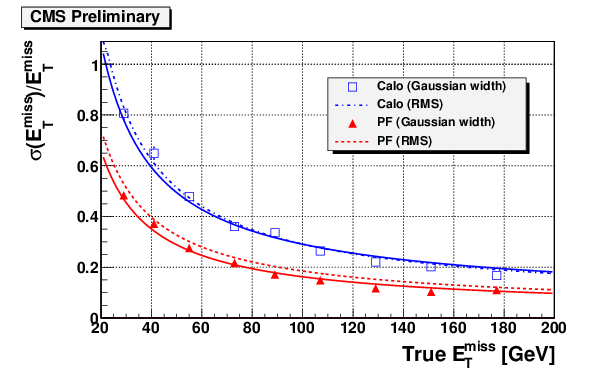
\includegraphics[width=0.48\textwidth]{objreconstruction/pics/true_met-a.png}
		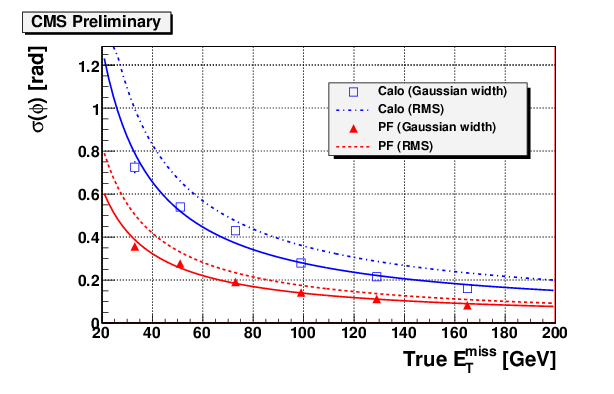
\includegraphics[width=0.48\textwidth]{objreconstruction/pics/true_met-b.png} 		
	\end{tabular}
	\caption{The energy and \ensuremath{\phi} resolution of the \met in simulation. Red triangles show the resolution for the PF approach. Blue squares show the resolution for the calorimetric approach. The full lines show the results of fits of the data points and the dashed lines show the results of fits of an alternative resolution measure \cite{CMS:2009nxa}}
	\label{fig:true_met}
\end{figure}

\clearpage